\documentclass[12pt]{article}

% Computational Physics by M. Newman
% Setup file for exercises

% Packages
\usepackage{mathpazo}
\usepackage{amsmath}
\usepackage{graphicx}
\usepackage{calrsfs}
\usepackage{fancyvrb}

% Formatting
\setlength{\textwidth}{17.5cm}
\setlength{\textheight}{24.0cm}
\setlength{\evensidemargin}{2.5cm}
\setlength{\oddsidemargin}{-0.6cm}
\setlength{\topmargin}{-2.3cm}
\setlength{\textfloatsep}{0pt}
\setcounter{secnumdepth}{0}
\renewcommand{\baselinestretch}{1.06}

% Macros
\newcommand{\dd}{\mathrm{d}}
\newcommand{\ii}{\mathrm{i}}
\newcommand{\e}{\mathrm{e}}
\newcommand{\half}{\tfrac12}
\newcommand{\av}[1]{\langle#1\rangle}
\newcommand{\var}{\mathop\mathrm{var}}
\newcommand{\Ord}{\mathrm{O}}
\renewcommand{\Re}{\mathop\mathrm{Re}\nolimits}
\renewcommand{\Im}{\mathop\mathrm{Im}\nolimits}
\newcommand{\mat}{\mathbf}
\renewcommand{\vec}{\mathbf}
\newcommand{\defn}{\textit}
\newcommand{\exskip}{\nopagebreak\medskip\noindent}
\newcommand{\pmstrut}{\rule{0pt}{13pt}}

% Environments
\newcounter{chapter}
\setcounter{chapter}{2}
\newcounter{exercise}
\renewcommand{\theexercise}{\arabic{chapter}.\arabic{exercise}}
\newenvironment{exercises}{\vspace{2ex plus0.5ex minus0.5ex}
  \renewcommand{\labelenumi}{\alph{enumi})}}%
    {\par\vspace{1ex plus0.5ex minus0.5ex}}
\newcommand{\exercise}{\refstepcounter{exercise}%
  \par\vspace{4ex plus1ex minus1ex}%
  \noindent\textbf{Exercise \theexercise: }}

\DefineVerbatimEnvironment{code}{Verbatim}{xleftmargin=\parindent}

\setcounter{chapter}{10}

\begin{document}

\noindent {\LARGE\textsc{Computational Physics}}\par
\bigskip
\noindent {\large\textsc{Exercises for Chapter \arabic{chapter}}}\par
\noindent\hrulefill

%%%%%%%%%%%%%%%%%%%%%%%%%%%%%%%%%%%%%%%%%%%%%%%%%%%%%%%%%%%%%%%%%%%%%%%
%%%                                                                 %%%
%%%     COMPUTATIONAL PHYSICS, M. NEWMAN, CHAPTER 10, EXERCISES     %%%
%%%                                                                 %%%
%%%%%%%%%%%%%%%%%%%%%%%%%%%%%%%%%%%%%%%%%%%%%%%%%%%%%%%%%%%%%%%%%%%%%%%

\begin{exercises}

%%% Exercise 10.1 %%%

\exercise \textbf{Rolling dice}
\begin{enumerate}\setlength{\itemsep}{0pt}
\item Write a program that generates and prints out two random
  numbers between 1 and 6, to simulate the rolling of two dice.
\item Modify your program to simulate the rolling of two dice a million
  times and count the number of times you get a double six.  Divide by a
  million to get the \emph{fraction} of times you get a double six.  You
  should get something close to, though probably not exactly equal
  to,~$\frac{1}{36}$.
\end{enumerate}


%%% Exercise 10.2 %%%

\exercise \textbf{Radioactive decay chain}

\exskip This exercise looks at a more advanced version of the simple
radioactive decay simulation in Example~10.1.

The isotope $^{213}$Bi decays to stable $^{209}$Bi via one of two different
routes, with probabilities and half-lives thus:
\begin{center}
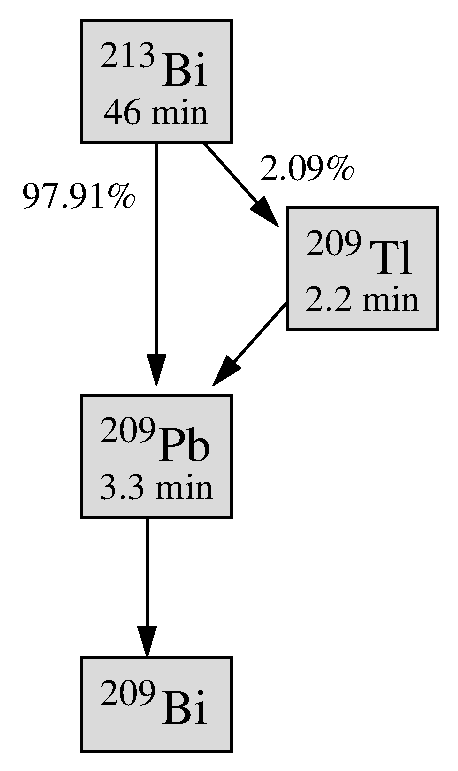
\includegraphics[width=4cm]{decaychain.eps}
\end{center}
(Technically, $^{209}$Bi isn't really stable, but it has a half-life of
more than $10^{19}$ years, a billion times the age of the universe, so it
might as well be.)

Starting with a sample consisting of $10\,000$ atoms of $^{213}$Bi,
simulate the decay of the atoms as in Example~10.1 by dividing time into
slices of length $\delta t=1\,$s each and on each step doing the following:
\begin{enumerate}\setlength{\itemsep}{0pt}
\item For each atom of $^{209}$Pb in turn, decide at random, with the
  appropriate probability, whether it decays or not.  (The probability can
  be calculated from Eq.~(10.3).)  Count the total number that decay,
  subtract it from the number of $^{209}$Pb atoms, and add it to the number
  of $^{209}$Bi atoms.
\item Now do the same for $^{209}$Tl, except that decaying atoms are
  subtracted from the total for $^{209}$Tl and added to the total for
  $^{209}$Pb.
\item For $^{213}$Bi the situation is more complicated: when a $^{213}$Bi
  atom decays you have to decide at random with the appropriate probability
  the route by which it decays.  Count the numbers that decay by each route
  and add and subtract accordingly.
\end{enumerate}
Note that you have to work up the chain from the bottom like this, not down
from the top, to avoid inadvertently making the same atom decay twice on a
single step.

Keep track of the number of atoms of each of the four isotopes at all times
for $20\,000$ seconds and make a single graph showing the four numbers as a
function of time on the same axes.


%%% Exercise 10.3 %%%

\exercise \textbf{Brownian motion}

\exskip Brownian motion is the motion of a particle, such as a smoke or
dust particle, in a gas, as it is buffeted by random collisions with gas
molecules.  Make a simple computer simulation of such a particle in two
dimensions as follows.  The particle is confined to a square grid or
lattice $L\times L$ squares on a side, so that its position can be
represented by two integers $i,j = 0\ldots L-1$.  It starts in the middle
of the grid.  On each step of the simulation, choose a random
direction---up, down, left, or right---and move the particle one step in
that direction.  This process is called a random walk.  The particle is not
allowed to move outside the limits of the lattice---if it tries to do so,
choose a new random direction to move in.

Write a program to perform a million steps of this process on a lattice
with $L=101$ and make an animation on the screen of the position of the
particle.  (We choose an odd length for the side of the square so that
there is one lattice site exactly in the center.)

Note: The \verb|visual| package doesn't always work well with the
\verb|random| package, but if you import functions from \verb|visual|
first, then from \verb|random|, you should avoid problems.


%%% Exercise 10.4 %%%

\exercise \textbf{Radioactive decay again}

\exskip Redo the calculation from Example~10.1, but this time using the
faster method described in the preceding section.  Using the transformation
method, generate 1000 random numbers from the nonuniform distribution of
Eq.~(10.5) to represent the times of decay of 1000 atoms of $^{208}$Tl
(which has half-life 3.053 minutes).  Then make a plot showing the number
of atoms that have not decayed as a function of time, i.e.,~a plot as a
function of~$t$ showing the number of atoms whose chosen decay times are
greater than~$t$.

Hint: You may find it useful to know that the package \verb|numpy| contains
a function \verb|sort| that will rearrange the elements of an array
in increasing order.  That is, ``\verb|b = sort(a)|'' returns a new
array~\verb|b| containing the same numbers as~\verb|a|, but rearranged in
order from smallest to largest.


%%% Exercise 10.5 %%%

\exercise
\begin{enumerate}\setlength{\itemsep}{0pt}
\item Write a program to evaluate the integral in Eq.~(10.22) using the
  ``hit-or-miss'' Monte Carlo method of Section~10.2 with $10\,000$ points.
  Also evaluate the error on your estimate.
\item Now estimate the integral again using the mean value method with
  $10\,000$ points.  Also evaluate the error.
\end{enumerate}
You should find that the error is somewhat smaller using the mean value
method.


%%% Exercise 10.6 %%%

\exercise Construct a general proof that the mean value method always does
better, or at least no worse, than the ``hit-or-miss'' method of
Section~10.2, as follows.
\begin{enumerate}\setlength{\itemsep}{0pt}
\item For an integral of the form~(10.27) with $f(x)\ge0$ everywhere in the
  domain of integration, show that Eq.~(10.23) can be rewritten as
\begin{displaymath}
I \simeq (b-a) H\av{s},
\end{displaymath}
where $H$ is the vertical height of the box enclosing the function to be
integrated (so that the box's area is $A=(b-a)H$) and $\av{s}$ is the
average of variables~$s_i$ defined such that $s_i=1$ if the $i$th point in
the Monte Carlo procedure was a ``hit'' (it fell below the curve of~$f(x)$)
and $s_i=0$ if it was a ``miss.''  Hence argue that the hit-or-miss method
will never be more accurate than the mean value method if the variance
of~$f$ in Eq.~(10.32) satisfies $\var(f) \le H^2\var(s)$.
\item Show that the variance of a single variable~$s_i$ is $\var(s) =
  p(1-p)$, where $p=I/A$ as in Section~10.2.  Show further that
  $p=\av{f}/H$ and $H^2\var(s) = \av{f}(H-\av{f})$ and thus that the
  hit-or-miss method will never be the more accurate method if
  $\av{f(f-H)}\le0$.  Given that the value of $f(x)$ never falls outside
  the interval from 0 to~$H$, prove that this last condition is always
  true.
\end{enumerate}
The hit-or-miss method can be extended to the case where $f(x)$ is not
always positive by adding a constant onto~$f(x)$ large enough to make it
always positive, calculating the integral of the resulting function, then
subtracting the constant again at the end.  The proof above can be extended
to this case by noting that the variance of~$f$ is unaffected by additive
constants, and hence the mean value method is always the more accurate of
the two integration methods for any function, positive or not.


%%% Exercise 10.7 %%%

\exercise \textbf{Volume of a hypersphere}

\exskip This exercise asks you to estimate
the volume of a sphere of unit radius in ten dimensions using a Monte Carlo
method.  Consider the equivalent problem in two dimensions, the area of a
circle of unit radius: \medskip
\begin{center}
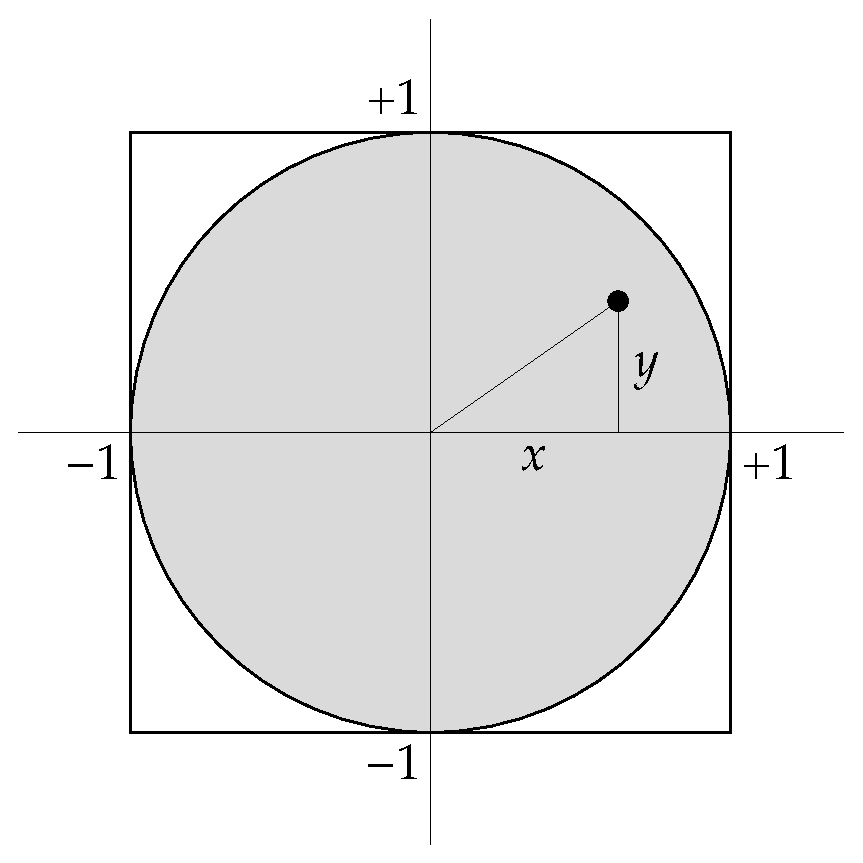
\includegraphics[width=7cm]{circle.eps}
\end{center}
The area of the circle, the shaded area above, is given by the integral
\begin{displaymath}
I = \iint_{-1}^{+1} f(x,y) \>\dd x\,\dd y,
\end{displaymath}
where $f(x,y)=1$ everywhere inside the circle and zero everywhere outside.
In other words,
\begin{displaymath}
f(x,y) = \biggl\lbrace\begin{array}{ll}
           1 &\qquad\mbox{if $x^2+y^2\le1$,} \\
           0 &\qquad\mbox{otherwise.}
         \end{array}
\end{displaymath}
So if we didn't already know the area of the circle, we could calculate it
by Monte Carlo integration.  We would generate a set of $N$ random points
$(x,y)$, where both $x$ and $y$ are in the range from $-1$ to~1.  Then the
two-dimensional version of Eq.~(10.33) for this calculation would be
\begin{displaymath}
I \simeq {4\over N} \sum_{i=1}^N f(x_i,y_i).
\end{displaymath}
Generalize this method to the ten-dimensional case and write a program to
perform a Monte Carlo calculation of the volume of a sphere of unit radius
in ten dimensions.

If we had to do a ten-dimensional integral the traditional way, it would
take a very long time.  Even with only 100 points along each axis (which
wouldn't give a very accurate result) we'd still have $100^{10} = 10^{20}$
points to sample, which is impossible on any computer.  But using the Monte
Carlo method we can get a pretty good result with a million points or so.


%%% Exercise 10.8 %%%

\exercise Calculate a value for the integral
\begin{displaymath}
I = \int_0^1 {x^{-1/2}\over\e^x + 1}\>\dd x,
\end{displaymath}
using the importance sampling formula, Eq.~(10.42), with $w(x)=x^{-1/2}$,
as follows.
\begin{enumerate}\setlength{\itemsep}{0pt}
\item Show that the probability distribution~$p(x)$ from which the sample
  points should be drawn is given by
\begin{displaymath}
p(x) = {1\over2\sqrt{x}}
\end{displaymath}
and derive a transformation formula for generating random numbers between
zero and one from this distribution.
\item Using your formula, sample $N=1\,000\,000$ random points and hence
  evaluate the integral.  You should get a value around~$0.84$.
\end{enumerate}


%%% Exercise 10.9 %%%

\exercise \textbf{The Ising model}

\exskip The Ising model is a theoretical
model of a magnet.  The magnetization of a magnetic material is made up of
the combination of many small magnetic dipoles spread throughout the
material.  If these dipoles point in random directions then the overall
magnetization of the system will be close to zero, but if they line up so
that all or most of them point in the same direction then the system can
acquire a macroscopic magnetic moment---it becomes magnetized.  The Ising
model is a model of this process in which the individual moments are
represented by dipoles or ``spins'' arranged on a grid or lattice: \medskip
\begin{center}
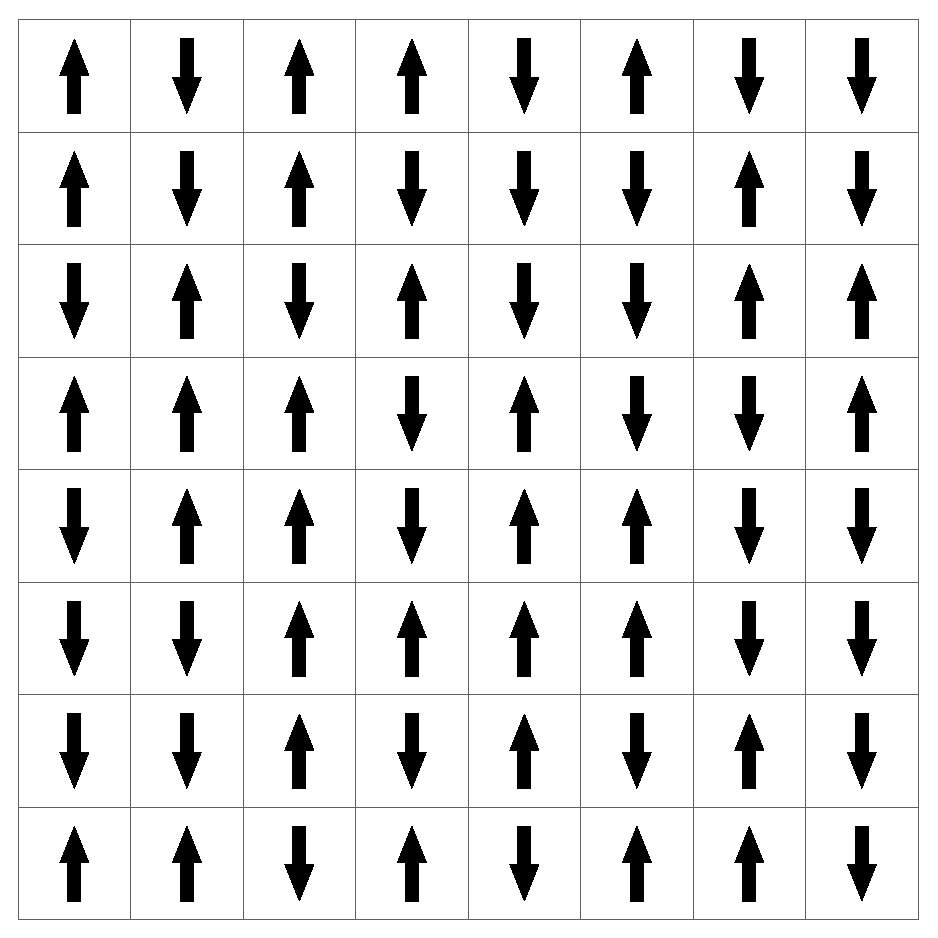
\includegraphics[width=5cm]{spins.eps}
\end{center}
In this case we are using a square lattice in two dimensions, although the
model can be defined in principle for any lattice in any number of
dimensions.

The spins themselves, in this simple model, are restricted to point in only
two directions, up and down.  Mathematically the spins are represented by
variables~$s_i=\pm1$ on the points of the lattice, $+1$ for up-pointing
spins and $-1$ for down-pointing ones.  Dipoles in real magnets can
typically point in any spatial direction, not just up or down, but the
Ising model, with its restriction to just the two directions, captures a
lot of the important physics while being significantly simpler to
understand.

Another important feature of many magnetic materials is that the individual
dipoles in the material may interact magnetically in such a way that it is
energetically favorable for them to line up in the same direction.  The
magnetic potential energy due to the interaction of two dipoles is
proportional to their dot product, but in the Ising model this simplifies
to just the product $s_is_j$ for spins on sites~$i$ and~$j$ of the lattice,
since the spins are one-dimensional scalars, not vectors.  Then the actual
energy of interaction is $-Js_is_j$, where~$J$ is a positive interaction
constant.  The minus sign ensures that the interactions are
\defn{ferromagnetic}, meaning the energy is lower when dipoles are
lined up.  A ferromagnetic interaction implies that the material will
magnetize if given the chance.  (In some materials the interaction has the
opposite sign so that the dipoles prefer to be antialigned.  Such a
material is said to be \defn{antiferromagnetic}, but we will not
look at the antiferromagnetic case here.)

Normally it is assumed that spins interact only with those that are
immediately adjacent to them on the lattice, which gives a total energy for
the entire system equal to
\begin{displaymath}
E = -J \sum_{\av{ij}} s_i s_j\,,
\end{displaymath}
where the notation~$\av{ij}$ indicates a sum over pairs~$i,j$ that are
adjacent on the lattice.  On the square lattice we use in this exercise
each spin has four adjacent neighbors with which it interacts.

Write a program to perform a Markov chain Monte Carlo simulation of
the Ising model on the square lattice for a system of $20\times20$ spins.
You will need to set up variables to hold the value $\pm1$ of the spin on
each lattice site, probably using a two-dimensional integer array, and then
take the following steps.
\begin{enumerate}\setlength{\itemsep}{0pt}
\item First write a function to calculate the total energy of the system,
  as given by the equation above.  That is, for a given array of values of
  the spins, go through every pair of adjacent spins and add up the
  contributions $s_is_j$ from all of them, then multiply by~$-J$.  Hint~1:
  Each unique pair of adjacent spins crops up only once in the sum.  Thus
  there is a term $-Js_1 s_2$ if spins 1 and~2 are adjacent to one another,
  but you do not also need a term $-Js_2 s_1$.  Hint~2: To make your final
  program to run in a reasonable amount of time, you will find it helpful
  if you can work out a way to calculate the energy using Python's ability
  to do arithmetic with entire arrays at once.  If you do the calculation
  step by step, your program will be significantly slower.
\item Now use your function as the basis for a Metropolis-style simulation
  of the Ising model with $J=1$ and temperature $T=1$ in units where the
  Boltzmann constant~$k_B$ is also~$1$.  Initially set the spin variables
  randomly to $\pm1$, so that on average about a half of them are up and a
  half down, giving a total magnetization of roughly zero.  Then choose a
  spin at random, flip it, and calculate the new energy after it is
  flipped, and hence also the change in energy as a result of the flip.
  Then decide whether to accept the flip using the Metropolis acceptance
  formula, Eq.~(10.60).  If the move is rejected you will have to flip the
  spin back to where it was.  Otherwise you keep the flipped spin.  Now
  repeat this process for many moves.
\item Make a plot of the total magnetization~$M=\sum_i s_i$ of the system
  as a function of time for a million Monte Carlo steps.  You should see
  that the system develops a ``spontaneous magnetization,'' a nonzero value
  of the overall magnetization.  Hint: While you are working on your
  program, do shorter runs, of maybe ten thousand steps at a time.  Once
  you have it working properly, do a longer run of a million steps to get
  the final results.
\item Run your program several times and observe the sign of the
  magnetization that develops, positive or negative.  Describe what you
  find and give a brief explanation of what is happening.
\item Make a second version of your program that produces an animation of
  the system using the \verb|visual| package, with spheres or squares of
  two colors, on a regular grid, to represent the up and down spins.  Run
  it with temperature~$T=1$ and observe the behavior of the system.  Then
  run it two further times at temperatures $T=2$ and $T=3$.  Explain
  briefly what you see in your three runs.  How and why does the behavior
  of the system change as temperature is increased?
\end{enumerate}


%%% Exercise 10.10 %%%

\exercise \textbf{Global minimum of a function}

\exskip Consider the function $f(x) = x^2 -
\cos 4\pi x$, which looks like this:
\bigskip
\begin{center}
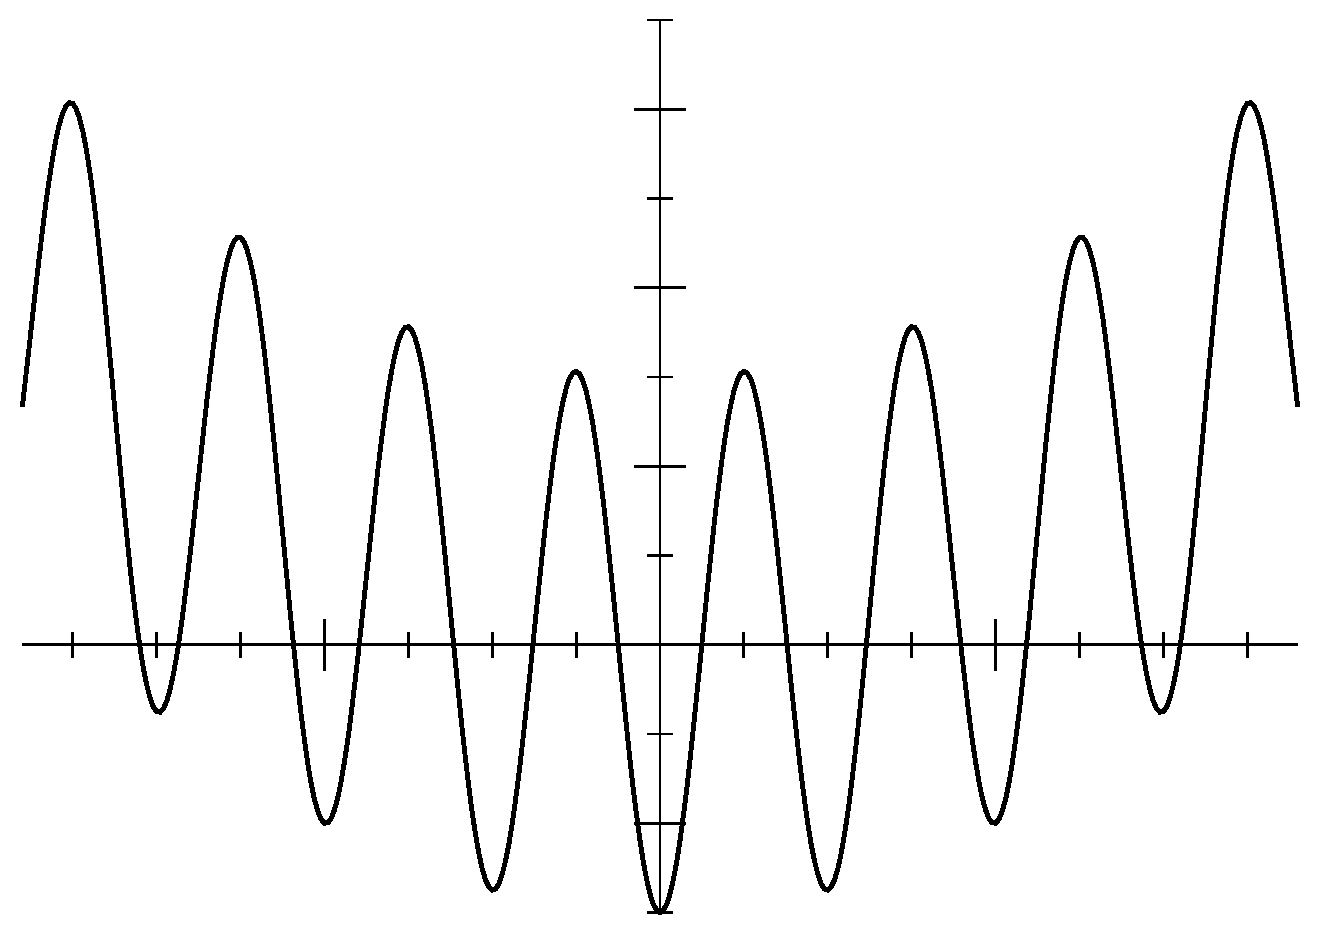
\includegraphics[width=7cm]{safx.eps}
\end{center}
Clearly the global minimum of this function is at $x=0$.
\begin{enumerate}\setlength{\itemsep}{0pt}
\item Write a program to confirm this fact using simulated annealing
  starting at, say, $x=2$, with Monte Carlo moves of the form $x\to
  x+\delta$ where $\delta$ is a random number drawn from a Gaussian
  distribution with mean zero and standard deviation one.  (See
  Section~10.1.6 for a reminder of how to generate Gaussian random
  numbers.)  Use an exponential cooling schedule and adjust the start and
  end temperatures, as well as the exponential constant, until you find
  values that give good answers in reasonable time.  Have your program make
  a plot of the values of $x$ as a function of time during the run and have
  it print out the final value of~$x$ at the end.  You will find the plot
  easier to interpret if you make it using dots rather than lines, with a
  statement of the form \verb|plot(x,".")| or similar.
\item Now adapt your program to find the minimum of the more complicated
  function $f(x) = \cos x + \cos \sqrt2x + \cos \sqrt3 x$ in the range
  $0<x<50$.
\end{enumerate}
Hint: The correct answer for part~(b) is around $x=16$, but there are also
competing minima around $x=2$ and $x=42$ that your program might find.  In
real-world situations, it is often good enough to find any reasonable
solution to a problem, not necessarily the absolute best, so the fact that
the program sometimes settles on these other solutions is not necessarily a
bad thing.


%%% Exercise 10.11 %%%

\exercise \textbf{The dimer covering problem}

\exskip A well studied problem in condensed matter
physics is the \defn{dimer covering problem} in which dimers,
meaning polymers with only two atoms, land on the surface of a
solid, falling in the spaces between the atoms on the surface and forming a
grid like this:
\medskip
\begin{center}
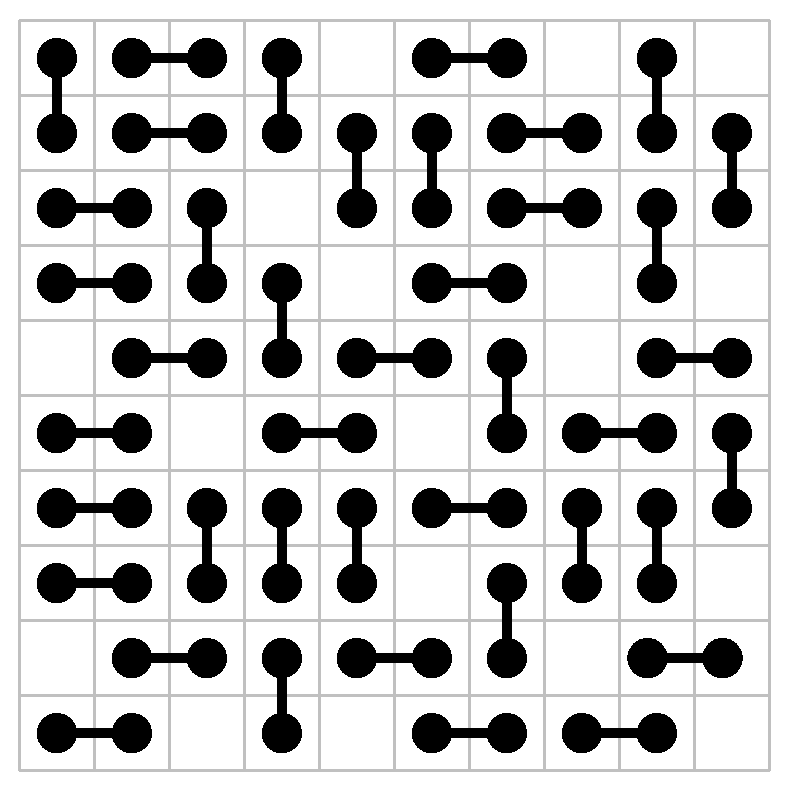
\includegraphics[width=5.5cm]{dimer.eps}
\end{center}
No two dimers are allowed to overlap.  The question is how many dimers we
can fit in the entire $L\times L$ square.  The answer, in this simple case,
is clearly $\half L\times L$, but suppose we did not know this.  (There are
more complicated versions of the problem on different lattices, or with
differently shaped elements, for which the best solution is far from
obvious, or in some cases not known at all.)
\begin{enumerate}\setlength{\itemsep}{0pt}
\item Write a program to solve the problem using simulated annealing
  on a $50\times50$ lattice.  The ``energy'' function for the system is
  \emph{minus} the number of dimers, so that it is minimized when the
  dimers are a maximum.  The moves for the Markov chain are as follows:
{\renewcommand{\labelenumii}{\roman{enumii})\ }
\begin{enumerate}\setlength{\itemsep}{0pt}\setlength{\parskip}{0pt}
\item Choose two adjacent sites on the lattice at random.
\item If those two sites are currently occupied by a single dimer, remove
  the dimer from the lattice.
\item If they are currently both empty, add a dimer.
\item Otherwise, do nothing.
\end{enumerate}}
Perform an animation of the state of the system over time as the simulation
runs.
\item Try exponential cooling schedules with different time
  constants.  A reasonable first value to try is $\tau=10\,000$ steps.  For
  faster cooling schedules you should see that the solutions found are
  poorer---a smaller fraction of the lattice is filled with dimers and
  there are larger holes in between them---but for slower schedules the
  calculation can find quite good, but usually not perfect, coverings of
  the lattice.
\end{enumerate}


%%% Exercise 10.12 %%%

\exercise \textbf{A random point on the surface of the Earth}

\exskip Suppose you wish to choose a random point on the surface of the
Earth.  That is, you want to choose a value of the latitude and longitude
such that every point on the planet is equally likely to be chosen.  In a
physics context, this is equivalent to choosing a random vector direction
in three-dimensional space (something that one has to do quite often in
physics calculations).

  Recall that in spherical coordinates $\theta,\phi$ the element of solid
  angle is $\sin \theta \>\dd\theta\>\dd\phi$, and the total solid angle in
  a whole sphere is~$4\pi$.  Hence the probability of our point falling in
  a particular element is
\begin{displaymath}
p(\theta,\phi)\>\dd\theta\>\dd\phi
  = {\sin \theta \>\dd\theta\>\dd\phi\over4\pi}.
\end{displaymath}
We can break this up into its $\theta$ part and its $\phi$ part thus:
\begin{displaymath}
p(\theta,\phi)\>\dd\theta\>\dd\phi
               = {\sin \theta \>\dd\theta\over2} \times{\dd\phi\over2\pi}
               = p(\theta)\,\dd\theta\times p(\phi)\,\dd\phi.
\end{displaymath}

\begin{enumerate}\setlength{\itemsep}{0pt}
\item What are the ranges of the variables $\theta$ and~$\phi$?  Verify
  that the two distributions $p(\theta)$ and $p(\phi)$ are correctly
  normalized---they integrate to~1 over the appropriate ranges.
\item Find formulas for generating angles~$\theta$ and~$\phi$ drawn from
  the distributions $p(\theta)$ and $p(\phi)$.  (The $\phi$ one is trivial,
  but the $\theta$ one is not.)
\item Write a program that generates a random~$\theta$ and~$\phi$ using the
  formulas you worked out.  (Hint: In Python the function
  \verb|acos| in the \verb|math| package returns the arc cosine in
  radians of a given number.)
\item Modify your program to generate 500 such random points, convert the
  angles to $x,y,z$ coordinates assuming the radius of the globe is~1, and
  then visualize the points in three-dimensional space using the
  \verb|visual| package with small spheres (of radius, say, 0.02).  You
  should end up with a three-dimensional globe spelled out on the screen in
  random points.
\end{enumerate}


%%% Exercise 10.13 %%%

\exercise \textbf{Diffusion-limited aggregation}

\exskip This exercise builds upon Exercise~10.3 on page~457.  If you have
not done that exercise you should do it before doing this one.

In this exercise you will develop a computer program to reproduce one of
the most famous models in computational physics, \defn{diffusion-limited
  aggregation}, or DLA for short.  There are various versions of DLA, but
the one we'll study is as follows.  You take a square grid with a single
particle in the middle.  The particle performs a random walk from square to
square on the grid until it reaches a point on the edge of the system, at
which point it ``sticks'' to the edge, becoming anchored there and
immovable:
\medskip
\begin{center}
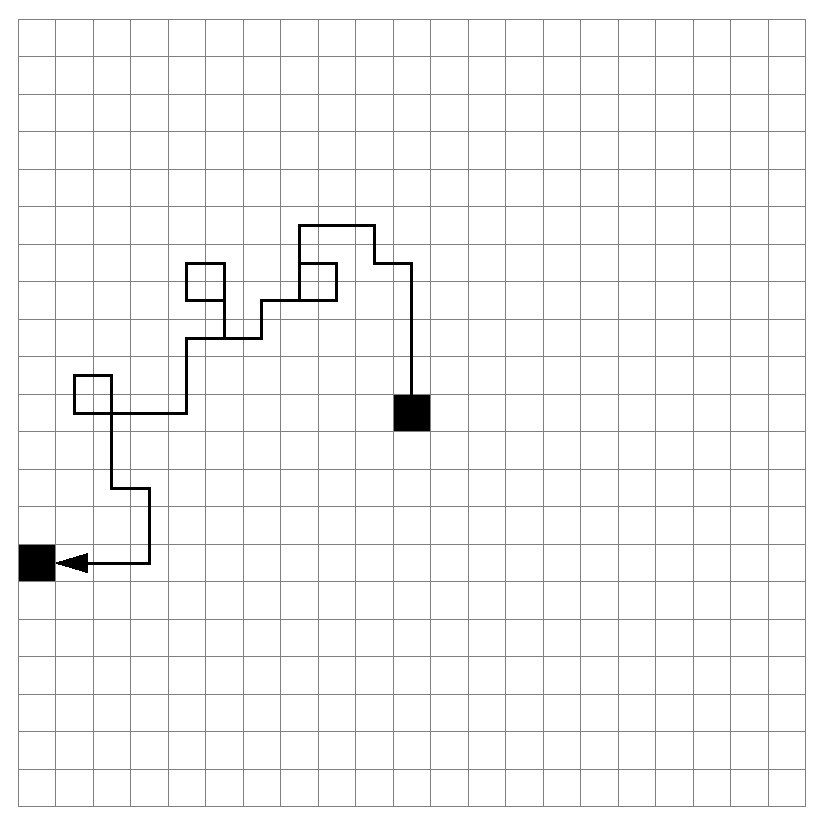
\includegraphics[width=7cm]{dla.eps}
\end{center}
Then a second particle starts at the center and does a random walk until it
sticks either to an edge or to the other particle.  Then a third particle
starts, and so on.  Each particle starts at the center and walks until it
sticks either to an edge or to any anchored particle.

\begin{enumerate}\setlength{\itemsep}{0pt}
\item Make a copy of the Brownian motion program that you wrote for
  Exercise~10.3.  This will serve as a starting point for your DLA program.
  Modify your program to perform the DLA process on a $101\times101$
  lattice---we choose an odd length for the side of the square so that
  there is one lattice site exactly in the center.  Repeatedly introduce a
  new particle at the center and have it walk randomly until it sticks to
  an edge or an anchored particle.

  You will need to decide some things.  How are you going to store the
  positions of the anchored particles?  On each step of the random walk you
  will have to check the particle's neighboring squares to see if they are
  outside the edge of the system or are occupied by an anchored particle.
  How are you going to do this?  You should also modify your visualization
  code from the Brownian motion exercise to visualize the positions of both
  the randomly walking particles and the anchored particles.  Run your
  program for a while and observe what it does.

\item In the interests of speed, change your program so that it shows only
  the anchored particles on the screen and not the randomly walking ones.
  That way you need update the pictures on the screen only when a new
  particle becomes anchored.  Also remove any \verb|rate| statements that
  you added to make the animation smooth.

  Set up the program so that it stops running once there is an anchored
  particle in the center of the grid, at the point where each particle
  starts its random walk.  Once there is a particle at this point, there's
  no point running any longer because any further particles added will be
  anchored the moment they start out.

  Run your program and see what it produces.  If you are feeling patient,
  try modifying it to use a $201\times201$ lattice and run it again---the
  pictures will be more impressive, but you'll have to wait longer to
  generate them.

  A nice further twist is to modify the program so that the anchored
  particles are shown in different shades or colors depending on their age,
  with the shades or colors changing gradually from the first particle
  added to the last.

\item If you are feeling particularly ambitious, try the following.  The
  original version of DLA was a bit different from the version above---and
  more difficult to do.  In the original version you start off with a
  single \emph{anchored} particle at the center of the grid and a new
  particle starts from a random point on the perimeter and walks until it
  sticks to the particle in the middle.  Then the next particle starts from
  the perimeter and walks until it sticks to one of the other two, and so
  on.  Particles no longer stick to the walls, but they are not allowed to
  walk off the edge of the grid.

  Unfortunately, simulating this version of DLA directly takes
  forever---the single anchored particle in the middle of the grid is
  difficult for a random walker to find, so you have to wait a long time
  even for just one particle to finish its random walk.  But you can speed
  it up using a clever trick: when the randomly walking particle does
  finally find its way to the center, it will cross any circle around the
  center at a random point---no point on the circle is special so the
  particle will just cross anywhere.  But in that case we need not wait the
  long time required for the particle to make its way to the center and
  cross that circle.  We can just cut to the chase and start the particle
  on the circle at a random point, rather than at the boundary of the grid.
  Thus the procedure for simulating this version of DLA is as follows:
{\renewcommand{\labelenumii}{\roman{enumii})\ }
\begin{enumerate}\setlength{\itemsep}{0pt}
\item Start with a single anchored particle in the middle of the grid.
  Define a variable~$r$ to record the furthest distance of any anchored
  particle from the center of the grid.  Initially $r=0$.
\item For each additional particle, start the particle at a random point
  around a circle centered on the center of the grid and having radius
  $r+1$.  You may not be able to start exactly on the circle, if the chosen
  random point doesn't fall precisely on a grid point, in which case start
  on the nearest grid point outside the circle.
\item Perform a random walk until the particle sticks to another one,
  except that if the particle ever gets more than $2r$ away from the
  center, throw it away and start a new particle at a random point on the
  circle again.
\item Every time a particle sticks, calculate its distance from the center
  and if that distance is greater than the current value of~$r$, update $r$
  to the new value.
\item The program stops running once $r$ surpasses a half of the distance
  from the center of the grid to the boundary, to prevent particles from
  ever walking outside the grid.
\end{enumerate}}
Try running your program with a $101\times101$ grid initially and see what
you get.
\end{enumerate}

\end{exercises}

\end{document}
